\chapter{Technical Proposal}\label{ch:solutionProposal}
This chapter will propose different types of sensors, wheel systems and energy sources, general materials and software.

\section{Sensors}
HADES will need sensors to scan its surrounding area for mapping and obstacle avoidance.

\subsection{Laser}
An autonomous vehicle will need to alter its path when objects occur. One of the most efficient ways for the vehicle to follow a trajectory is with structured light.\\This light will project a triangular image for the image sensor processor to process. It will then derive the range and bearing for the illuminated object from the beam of structured light and match it to the current position of the vehicle\cite{Lasers}.


\subsection{Radar}
Radars use a highly concentrated radio wave, if there's any obstacles on its way, it will reflect electromagnetic energy. The sensor will then pick up the signalling energy and measure the time spent on getting the "echo" back\cite{Radar}.

The further away the transmission has to be sent, the lower the frequency has to.
Satellites are typically using C-band ( 300 MHz - 1 GHz ). 
For avoidance on the other hand, it will be of utmost importance for us to get higher frequencies, since the system has to maneuver at high accuracy. This frequency for avoidance will generalized be at I- or J-band (8-12 GHz)\cite{RadarTutorial}.

%\begin{figure}[h]
    %\centering
   % 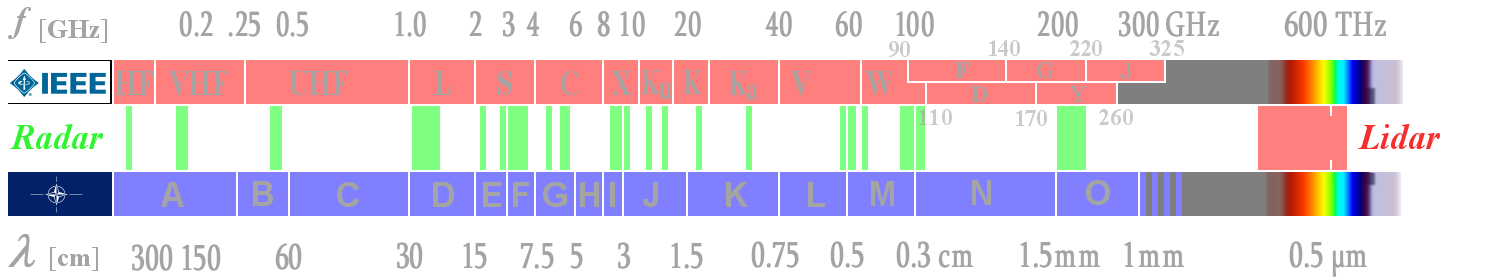
\includegraphics[width=\textwidth]{figures/radarfrequencies.png}
  %  \caption{Radar Frequencies \cite{RadarTutorial}}
 %   \label{fig:radarfrequencies.png}
%\end{figure}


\subsection{LIDAR}
Since the most common platforms for LIDAR is airplanes, this remote-sense and GPS uses the light from the surface of earth to reflect and then scan the surroundings. This method is used for both its accuracy and differentiating man-made versus nature structures\cite{LIDAR}.

\subsection{Cameras (RGB-D)} \label{ch:CameraRGB}

Some RGB-D uses a night-vision camera and a laser that produce a unique cloud of points. The camera triangulates the distance to the different points from the laser. This triangulation can then be translated into map with depth, that will let the robot determine the distance to different objects. 
A downside to the night vision RGB-D cameras is that it does not work in sunlight. This is because the infrared light rays interferes with the camera\cite{Cameras}.

\subsection{Ultrasonic sensors}
Ultrasonic sensors uses sound waves to measure distance to various obstacles. One part of the sensor called a transducer, emits a sound wave that hits the surface, bounces back and gets picked up by the receiver. 
%To calculate how far away a set of objects is, the wave formula is needed to calculate the velocity of the wave. Lambda is the wavelength, f is the frequency of the wave and v is the velocity.
%\begin{equation}\label{eq:ultrasonic01}
 %   v= \lambda \cdot f
%\end{equation}
%For calculating distance(d) back and forwards the velocity is needed and the time (t) for the signal to be sent and received. 
%\begin{equation}\label{eq:unltrasonic02}
 %  d=t\cdot v 
%\end{equation}
%The distance has to be halved, because the time is from the transducer to the receiver.
%\begin{equation}\label{eq:unltrasonic03}
 %  DTO=d/2
%\end{equation}
Ultrasonic sensors is a cheap solution, but sound can deflect different from some surfaces, which is a problem. They can also be sensitive to noise in the signal and the sensor does not have a good sense of direction because of the sound wave is fan-like shaped. All this can be overcome by using an array of ultrasonic sensors to help build up a more accurate map, by having multiple inputs from the array\cite{Ultrasonicsnesor}.
%\newpage